\documentclass[../ClassicThesis.tex]{subfiles}
\begin{document}

% ************************************************
\chapter{Introduction}
\label{ch:introduction}
% ************************************************

\section{Fabrication Machines Enable Anyone to Bring Their Ideas to Life}

\note{maybe subdivide this package?}
% people are awesome -> ideas
% bringing ideas to live -> back in time -> difficult
% transition, changes now
% machines -> plug into your computer -> take over fabrication for you

People always had ingenious ideas. Though, back in time it was
difficult bringing these ideas to life. For example in the field of
engineering, when one has an idea how airplanes fly better
(Figure~\ref{fig:intro-ideas:plane}). Or ideas concerning an creative
process, like a fashion line for shoes which offer correct fit to the
shape of the feet of its wearer (Figure~\ref{fig:intro-ideas:shoe}).
Even in health care broad ideas evolve. In 2013 Jake Evill presented
\name{Cortex}, a customizable plaster that is \enquote{fully
  ventilated, super light, shower friendly, hygienic, recyclable and
  stylish}\footnote{\url{http://www.evilldesign.com/cortex}}, see
Figure~\ref{fig:intro-ideas:plaster}. \note{give sources of images.
  how to give sources? as footnote??}

\begin{figure}[h]
  \centering
  \begin{subfigure}[b]{0.321\textwidth}
    \centering
    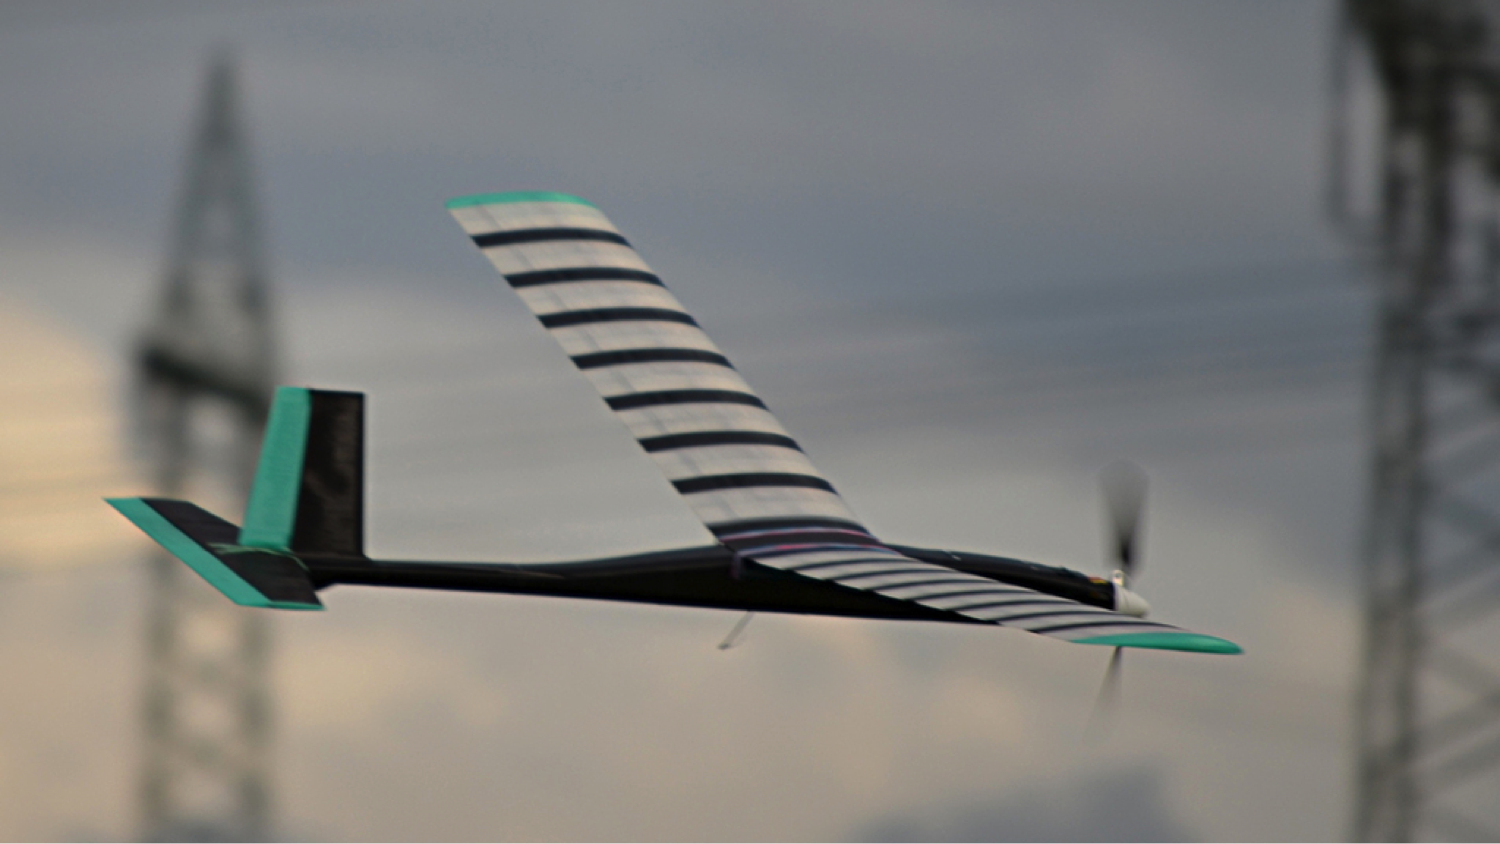
\includegraphics[width=\textwidth]{01-intro-plane}
    \caption{A self-fabricated model airplane.}
    \label{fig:intro-ideas:plane}
  \end{subfigure}
  \begin{subfigure}[b]{0.321\textwidth}
    \centering
    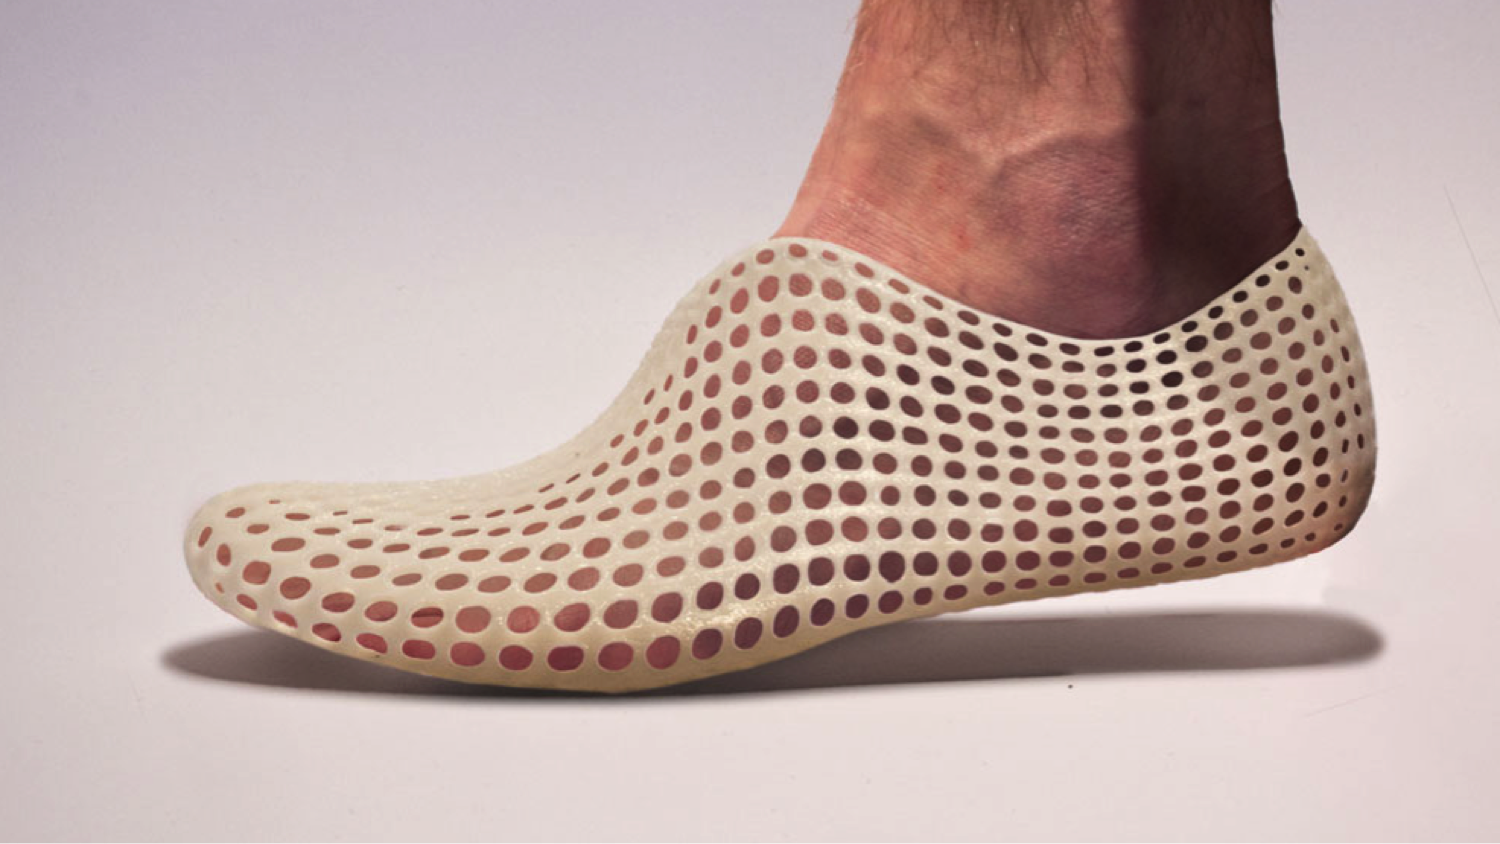
\includegraphics[width=\textwidth]{01-intro-shoe}
    \caption{A shoe with correct fit to its wearer.}
    \label{fig:intro-ideas:shoe}
  \end{subfigure}
  \begin{subfigure}[c]{0.321\textwidth}
    \centering
    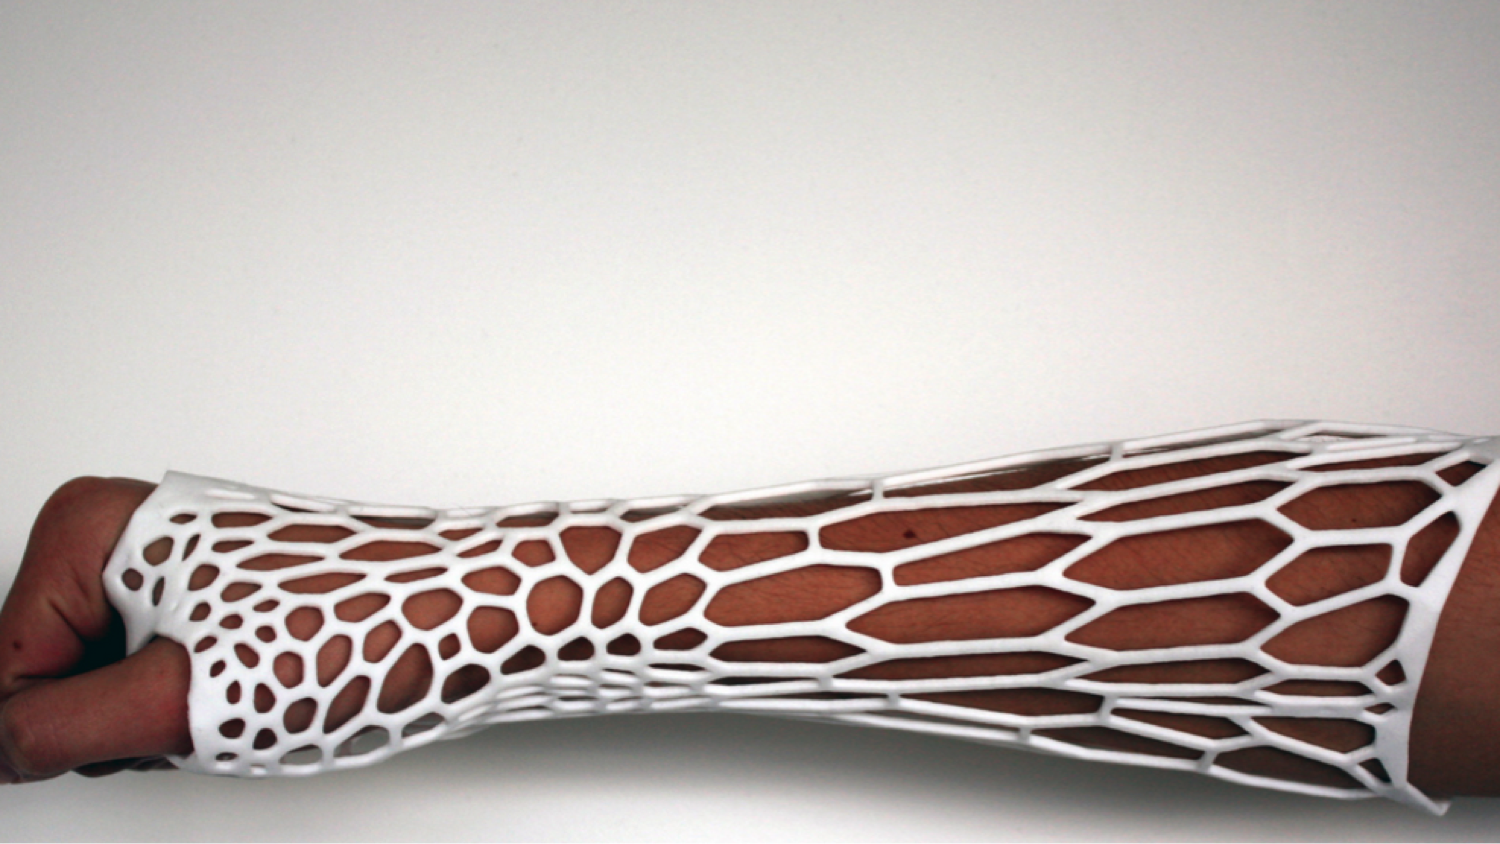
\includegraphics[width=\textwidth]{01-intro-plaster}
    \caption{\name{Cortex}, a fully ventilated plaster.}
    \label{fig:intro-ideas:plaster}
  \end{subfigure}
  \caption{With fabrication machines, broad ideas come to life.}
  \label{fig:intro-ideas}
\end{figure}

The way ideas are turned into reality is changing. Today, machines
exist that we can plug into our computer that will take over the
fabrication of objects. Thus, we can fully concentrate on the ideas
instead of requiring and acquiring additional skills to actually
fabricate.

% one of theses machines => 3d printer
% market -> growing, machines more and more affordable
% layerwise plastik materials, free forms, easy to use -> button click -> object out.
% but: limitations -> slow, material (lose structure/ beauty)

Such a fabrication machine is a 3D printer. 3D printing is an emerging
technology spreading across the consumer market. According to
\name{Wohlers Associates}, in the year 2015 the 3D printing market was
worth 6.5 billion USD. Their prognosis estimates a roughly 300\%
growth in the next five years\cite{wohlers-market}. With 3D printers
literally any user can produce any free-form object with a button
press. A common technique in 3D printing is fused deposition modeling
(FDM)\cite{}\note{source that FDM is common}. With the FDM technique,
thermoplastic material is heated and then pressed through a nozzle,
mounted on a print head. Thus, layer by layer material is extruded to
create three dimensional objects\cite{}\note{source thats how FDM
  works}.

Though 3D printing brings a substantial progress in the field of
fabrication, it shows two flaws: 3D printing is slow and 3D printing
is limited in its materials. Even small models need a couple of hours
to be printed. The miniature bird house in Figure~\ref{}\note{figure}
printed for three hours\footnote{Printed with the \name{Ultimaker~2+},
  \url{https://ultimaker.com/en/products/ultimaker-2-plus}}. In its
original dimensions it needs about two days of printing
time\footnote{Estimated with the \name{Cura~2} 3D~printer software,
  \url{https://ultimaker.com/en/products/cura-software}}. The FDM
technique requires material to be pushed through a nozzle. Thus, the
material is melted and loses its original structure and
characteristics.

% other machine, our target machine -> laser cutter
% cutting materials from a cut plan (typically svg file)
% 2d shapes/ plates
% assembled to objects
% materials like wood, acryllic, textiles, metal or stone
% laser cutter -> low-fi fabrications
% faster than printer
% market laser cutters is coming

% you
% can build 3d things from the laser cutter as well. though not
% freeform, but it is possible iterating on functional objects -> drone
% original materials can be used -> designer glasses but 2 challenges:

Another fabrication machine is the laser cutter, shown in
Figure~\ref{}\note{figure}. A laser traces the outlines of a planar
cutting plan, so actual plates are cut from the materials
(Figure~\ref{}\note{figure}). Such materials are wood or acrylic.
High-performance devices can cut textiles, metals or stone. The laser
cutter is fast and preserves the original structure of the used
materials. Figure~\ref{} and Figure~\ref{} show how the cut-out plates
are assembled to a three dimensional object in several minutes. With a
laser cutter, we perform low fidelity fabrications. Low-fi means, we
produce functional objects that fulfill their purpose, but lack the
amount of detail a full-fledged product would have. Nonetheless, we
can iterate several times a day on our object to produce better
results. In comparison to 3D printing, we can use the time more
efficiently. Such a functional object is a quadcopter produced from
wood, shown in Figure~\ref{}\note{figure}. With a laser cutter, we can
also produce decorative objects (Figure~\ref{}\note{figure}). Here, we
benefit from the original characteristics of the materials.

% need to assemble. spatial orientation. need to know where plates from the cutting plan will resemble on final model.
% need knowledge about materials. knowledge a carpenter or craftsman has. fingerjoints for example
% manual drafting of cutting plans for large objects -> difficult
% each connection must be placed exactly, on millimeter, others plates stuck or fall apart

When creating three dimensional objects with a laser cutter, users
face two challenges: They need a vast amount of spatial orientation
and they need craft men's knowledge about the used materials. The
final object has to be assembled from the cut-out plates. The user has
to know, where the plates will resemble on the objects in 3D space.
Then, the user has to attach the plates to each other. In the case of
wooden material, this would be typical knowledge of a carpenter. In
Figure~\ref{}\note{figure} we combined the plates of a bird house with
finger joints. When creating cutting plans manually for larger
objects, a lot of detailed work is required. All connections have to
be positioned perfectly, otherwise the plates stuck or fall apart
during assembly.

% we aim to make 3d model fabrication with laser cutter easy. using its pros in time, material. improving the creation of cut plans
% we present software system platener
% similar intuitive approach as with 3d printing. start from 3d model. user knows how results will look lik.
% our software converts 3d model to a suitable cutting plan.
% analyzes geometries -> approximating a model with plates (different techniques we elaborate on in this thesis)
% putting plates together (software knows which materials -> allowing to place finger joints calibrated for the laser cutting, allowing bends).

In this thesis, we present a solution which enables users to produce
three dimensional objects with a laser cutter. We improve the creation
process of cutting plans, so that users do not require any additional
skills. Similar to 3D printing, we start out with a 3D model. Every
user can imagine from the model, how the final object will look like.
Our software system {\platener} converts the 3D model to a 2D cutting
plan. {\platener} analyzes the geometries and approximates the model
with plates. The software also knows which materials we want to use.
Thus, it generates all connection between the plates automatically.
The connections are nicely calibrated, meaning all plates fit tight
together without using any glue or other means of attachment. With our
software, users benefit from the advantages of a laser cutter, namely
speed and choice of materials. Meanwhile our software takes the burden
from the user to create cutting plans manually.

% in this thesis we talk about:

% architecure
% data structures
% approximation of high-res models
% plate finding
% plate joining
% advanced analysis and conversion technique (future work)

\note{cross refs}
We present our system architecture in Chapter~\ref{}. Then, we give an
overview of the most important data structures in Chapter~\ref{}. From
Chapter~\ref{} to Chapter~\ref{} we explain the conversion process of
3D~models to 2D~cutting plans. We elaborate on future work and
improvements of our system in Chapter~\ref{}.


\end{document}

%%% Local Variables:
%%% mode: latex
%%% TeX-master: "../ClassicThesis"
%%% TeX-command-extra-options: "-shell-escape"
%%% End:
